\documentclass[a4paper]{article}
\usepackage[nottoc]{tocbibind}
\usepackage[utf8]{inputenc}
\usepackage{listings}
\usepackage{graphicx}
\usepackage{float}

\title{Prevent overcrowding in exhibitions using FogFlow to distribute people}
\author{Lorenzo Siega Battel\\Politecnico di Milano\\lorenzo.siega@mail.polimi.it}
\date{}

\begin{document}
\maketitle
\newpage
\tableofcontents
\newpage

\section{Introduction}
\subsection{Introduction}
This document aims to provide an outlook on FogFlow framework and then analyse its adaptability in a real world application.\\
In the first half of this document we will see the goals at which FogFlow aims and then, in the second half, what is capable of doing by applying it to a research problem.

\subsection{Effort}
To develop this project some changes have been made, including modification of the FogFlow's core components. In this was put the majority of the effort spent on the project, also trying to integrate FogFlow with other tools. This underlines a substantial immaturity of the project but, over time, it will be resolved as the project may attract other developers.

\newpage
\section{FogFlow as...}
In this section we will see the most important features that FogFlow offers to developers.

\subsection{Context driven IoT framework}
FogFlow is an context driven IoT framework mostly written in Go. Context driven means that FogFlow is able to orchestrate data processing basing its decisions on three types of contexts:

\begin{itemize}
    \item System context: available resources which are changing over time.
    \item Data context: the structure and registered metadata of available data, including both raw sensor data and intermediate data.
    \item Usage context: high level intents defined by all different types of users (developers, service consumers, data providers) to specify what they want to achieve.
\end{itemize}
By taking advantage of these three kinds of context, FogFlow is able to orchestrate IoT services in a more intelligent and automatic manner.\\\\
To better understand what a context could be, let me give you the following example:\\
You can think of multiple sensors that count people who are entering in a building, a single sensor can produce a context called “Ingoing at entrance 2-A” while all the sensors placed at the entrances of a building can produce a context called “People flow in building 2”.\\
FogFlow can handle this different types of context producing different other context updates based on where they will be "deployed". For example it can reduce the flow at a single entrance or cut it when a building is becoming full of people.\\\\
This behaviour is also enabled by introducing a new layer, namely IoT Discovery, which provides a update summary of available entity data on all brokers. As compared to event or topic based orchestration, the context-based orchestration in FogFlow is more flexible and more light-weight. This is because the orchestration decisions in FogFlow can be made based on aggregated context, without reading through all involved data streams.
\begin{figure}[H]
    \centering
    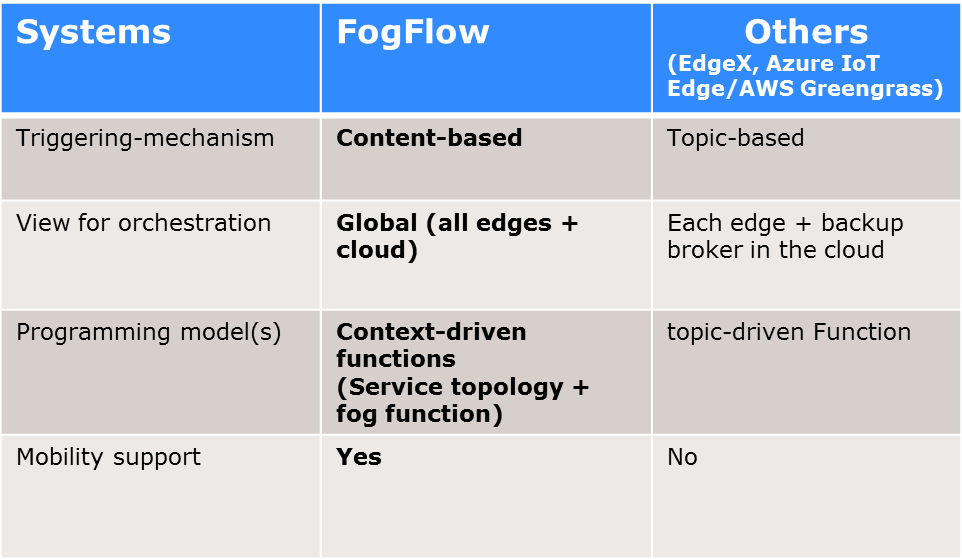
\includegraphics[width=0.7\textwidth]{Images/comparison.png}
    \caption{Comparison between FogFlow and other IoT platforms}
\end{figure}{}

\subsection{Serverless and edge computing}
FogFlow merges two paradigm: serverless computing and edge computing. This allows developers to create new kinds of triggers, by defining them on context updates and then let the computation executes on geographically distributed workers.\\
These workers can be deployed near the devices that produce the data allowing a low latency response and a reduction in terms of bandwidth.\\\\
In particular, code is executed inside a Docker container and the relative image must be published on Docker Hub. Beside some obvious privacy concerns, this kind of approach can be very useful to better manage instances.
\begin{figure}[H]
    \centering
    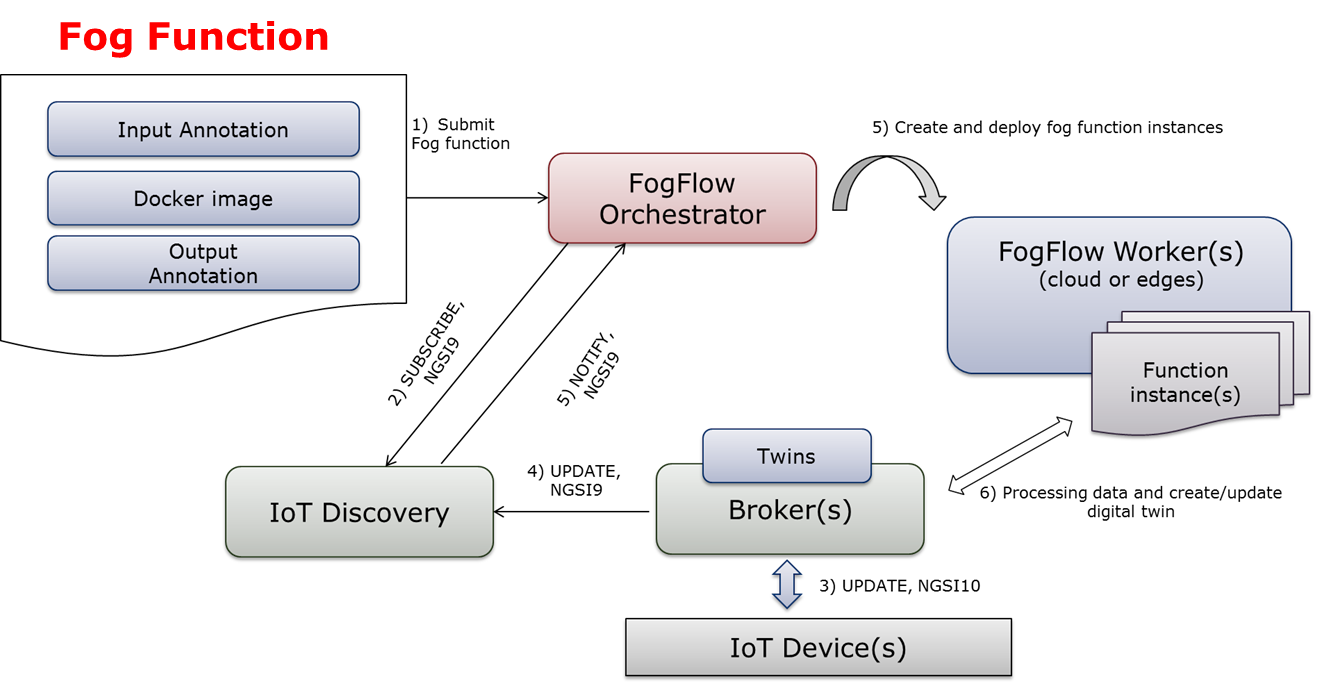
\includegraphics[width=0.7\textwidth]{Images/function-orchestration.png}
    \caption{FogFlow system structure}
\end{figure}{}

\subsubsection{Operator and Fog Function}
FogFlow enables serverless edge computing, meaning that developers can define and submit a so-called fog function and then the rest will be done by FogFlow automatically, including:
\begin{itemize}
    \item Triggering the submitted fog function when its input data are available
    \item Deciding how many instances to be created on workers according to its defined granularity
    \item Deciding where to deploy the created instances
\end{itemize}{}
The instances in the above text refer to the task instances which run a processing logic within them and this processing logic is given by the operator.

\subsection{Location based discovery}
In FogFlow is mandatory to have a low latency and distributed computation. To achieve that a component called "IoT discovery", having a system level point of view, can provide the best suitable broker to each component.\\
Also, as previously said, it can provide an aggregated context that only a system level entity might has.

\begin{figure}[H]
    \centering
    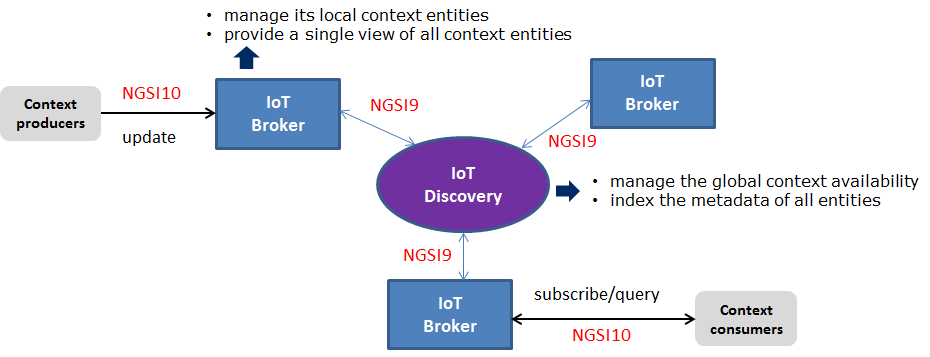
\includegraphics[width=0.7\textwidth]{Images/distributed-brokers.png}
    \caption{IoT discovery}
\end{figure}{}

\newpage
\section{The research problem}
\subsection{Abstract}
The organizers of an exhibition with several booths are trying to avoid overcrowded booths so visitors could be distributed smoothly and enjoy the exhibition. They mount sensors at each booth so to know the number of people currently at each booth. Each booth has an electrical board which, based on the information from other booths their distance, suggests visitors the closest booth to visit next in a way that the population is smoothly distributed. The overall number of visitors of each booth is reported to the cloud for information aggregation to be queried for the crowded time of the day.

\subsection{Technical challenges}
In this document we will address the problem by leaving the choice of the sensor and the algorithm to the final people who finally implement the system.\\
During the development of such a system two main problems will have to be addressed:
\begin{itemize}
    \item Required analysis effort: As we have to analyze a stream of data from a large number of sensors, we can't compute it on a centralized component.
    \item Algorithm: Algorithm works on the entire set of booths and triggering it on each update received from a booth, as FaaS computing does, will generate an high computation and data load.
\end{itemize}{}
FogFlow can address to both problems, by filling these gaps (for a more in-depth explanation please refer to the cited document):
\textit{
\begin{quote}
    \begin{enumerate}
        \item[G2] Function triggering: from per event to per selected entities: In existing serverless computing frameworks, functions are invoked per event with limited execution time and memory size. This is not suitable for data-intensive IoT services.
        \item[G3] Function execution: from data $\rightarrow$ code or code $\rightarrow$ data to code $\leftrightarrow$ data: Existing serverless computing frameworks separate data management from the function execution environment, always moving data into the execution environment for function execution (data to code pattern). On the other hand, existing fog computing frameworks such as Azure IoT Edge move cloud functions to the data located at the edges.
        \item[G4] Function composition: from event-oriented or edge-oriented to data-centric: 
        In existing serverless computing frameworks such as OpenWhisk, service developers need to customize a series of event triggers and rules to link multiple functions together. Existing fog computing frameworks allow service developers to link functions at each edge by manually configuring the topic-based data routing path between them.
    \end{enumerate}{}
    \cite{cheng2019fog}
\end{quote}
}
\subsection{Context producers and context consumers}
In FogFlow, as it is a data-centric framework, our first goal is to produce data, process it and then utilize that data to make decisions or let others do that.\\
During the development of this project, not having to deal with a real situation, data is produced by a web dashboard written in Angular.js and a Node.js server.

\begin{figure}[H]
    \centering
    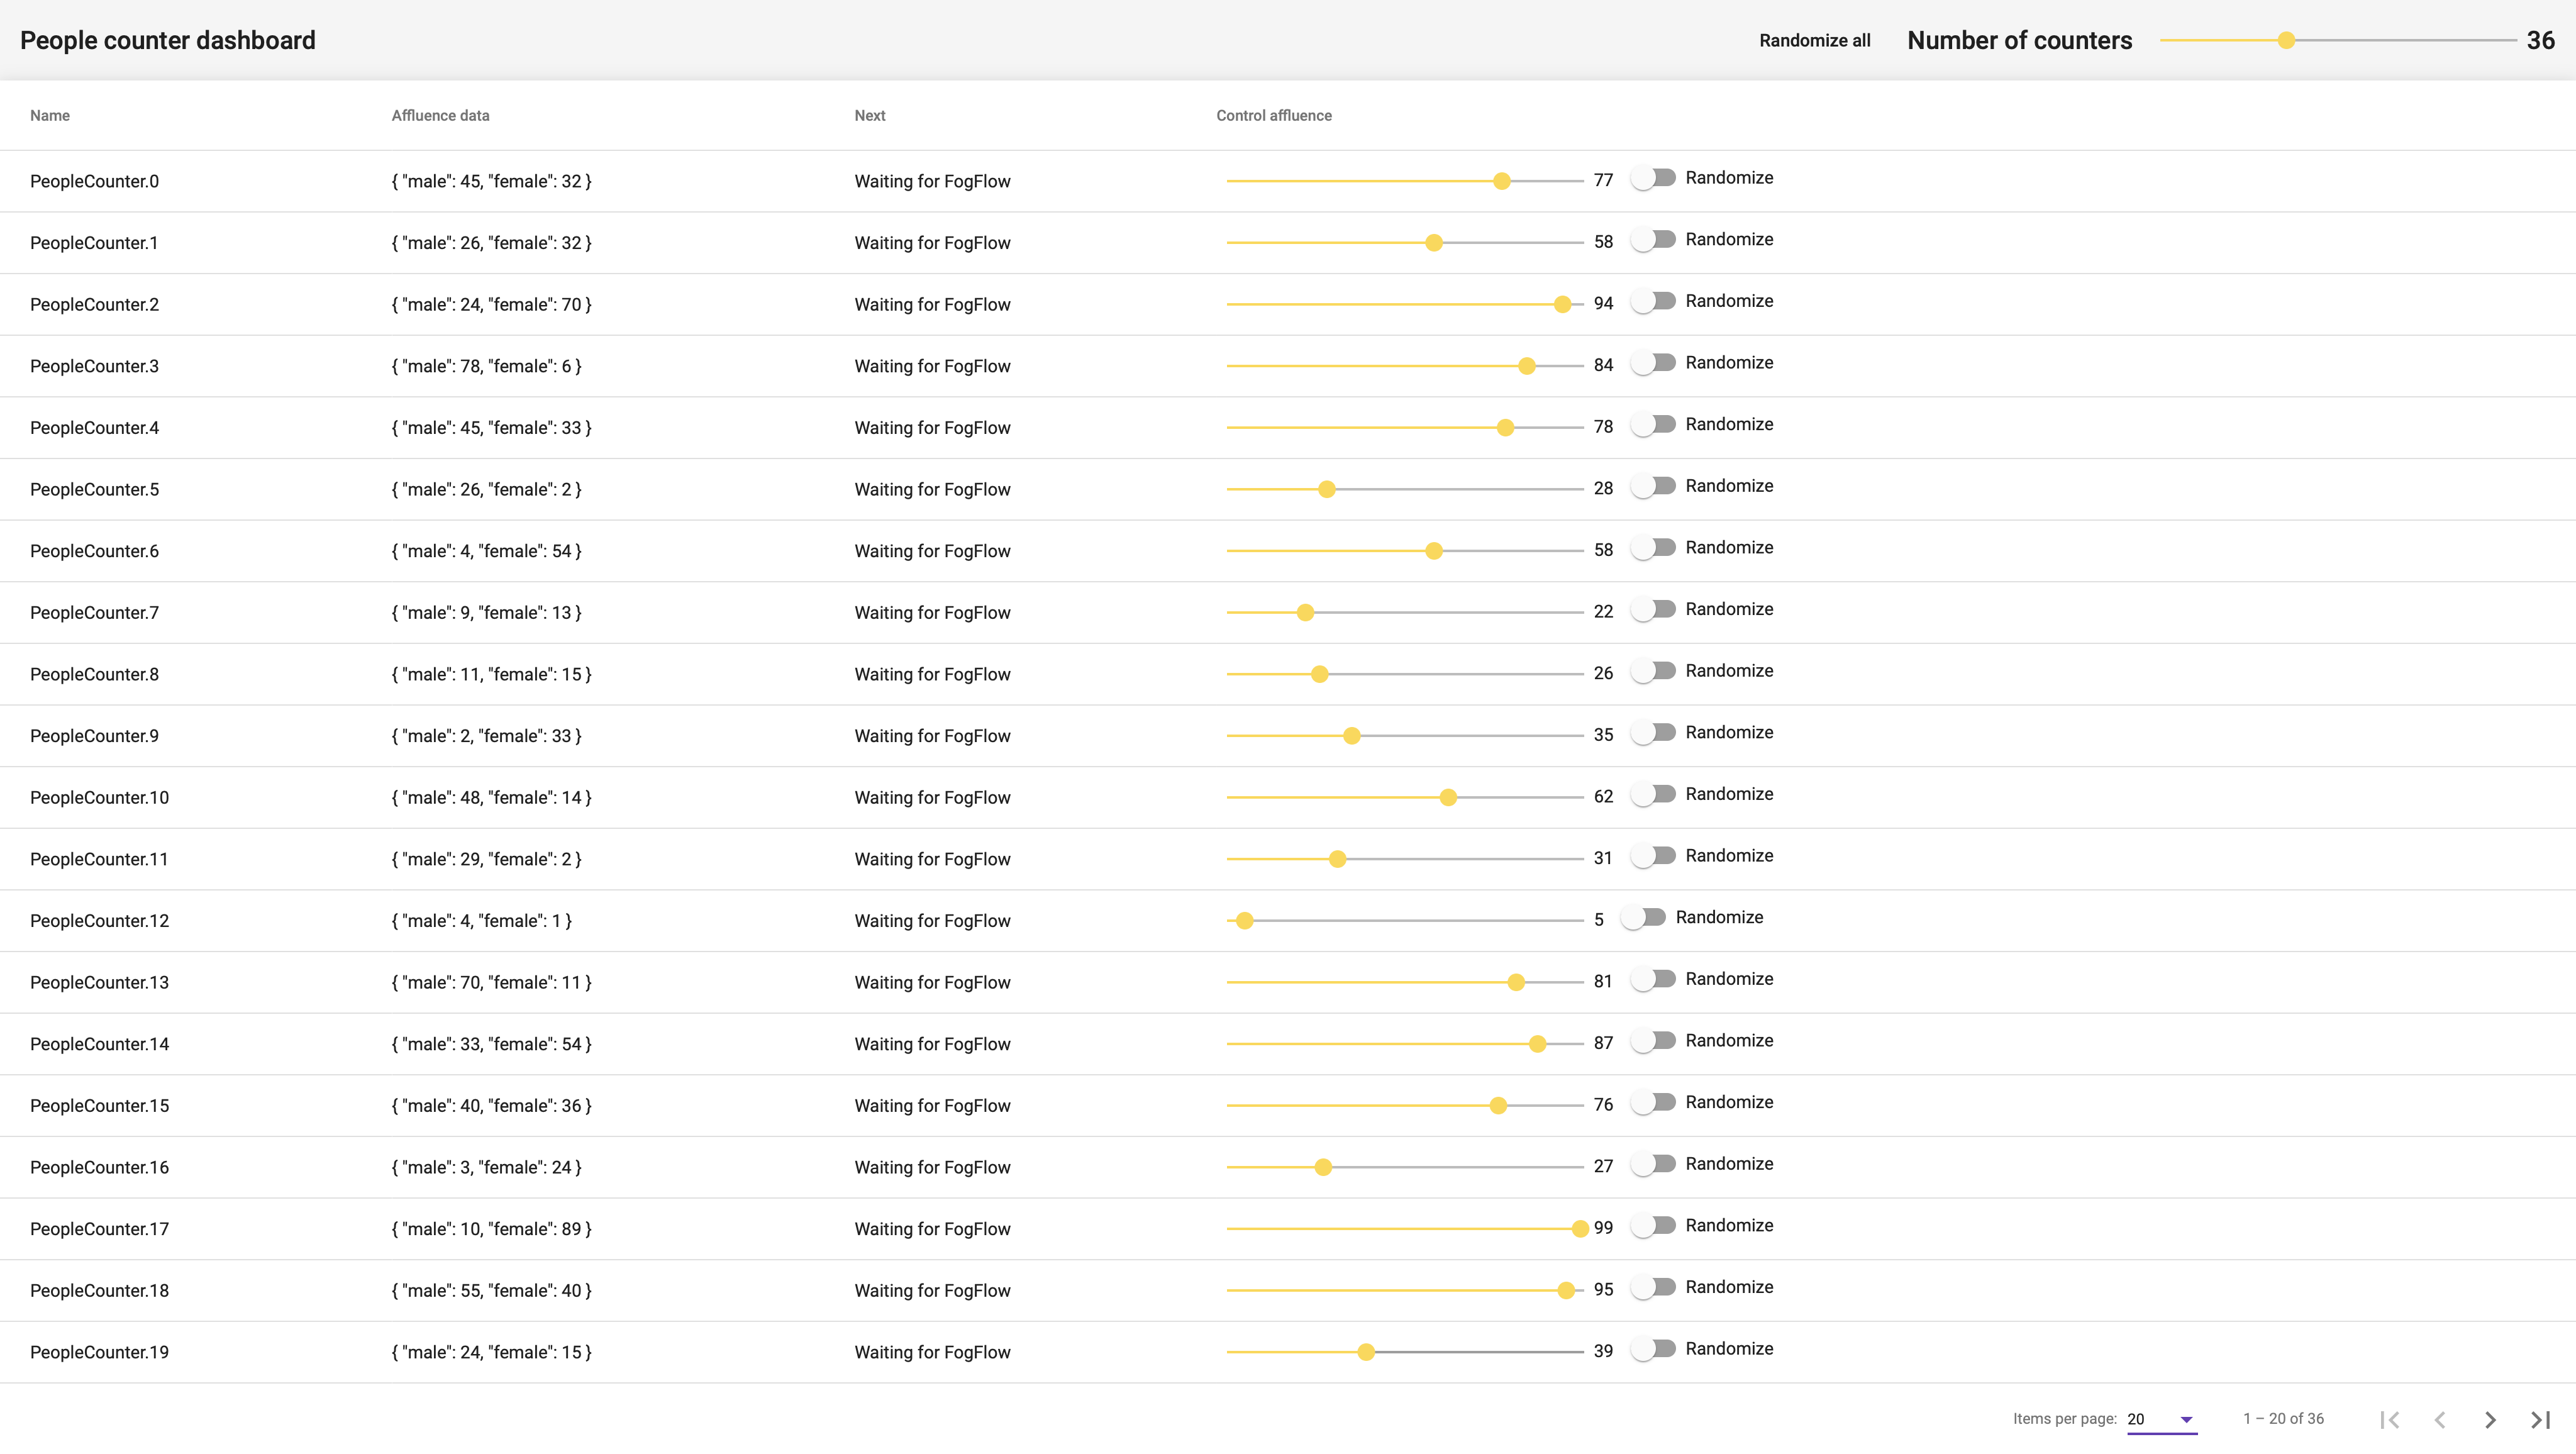
\includegraphics[width=\textwidth]{Images/web_dashboard.png}
    \caption{Web dashboard to produce sensor data}
\end{figure}{}

\subsubsection{Context producer aka the sensor}
We cannot know \textit{a priori} the pyhisical structure of an exhibition so we do not provide any constraint on the type of the sensor.
Sensor's data will be processed on site and then sent to the nearest broker adopting its NGSI10 APIs.

\subsubsection{Context consumer aka the electronic board}
As for the sensor we cannot know how informations will be displayed so an intermediate device is needed to receive data from FogFlow and then show it.\\
It will expose an HTTP server which will be used by the broker to send context updates.

\subsection{Data querying and visualization}
To better provide insights on how people move through the exposition and to allow the organizers to perform queries on the data, a scraping tool is needed.
Prometheus is the best choice for two reasons:
\begin{itemize}
    \item It allows users to perform queries on its data directly and not by using other tools
    \item It's widely supported by data visualization tools like Grafana
\end{itemize}{}
Perhaps the broker must be modified to expose a web service that matches the syntax accepted by Prometheus.
Please notice that from now on we will see three values for each counter (count, male and female). These values are chosen by the developer (the broker exposes the values uploaded by the sensors) and so they are not fixed.

\begin{lstlisting}
PeopleCounter_1{name="count"} 56
PeopleCounter_1{name="male"} 37
PeopleCounter_1{name="female"} 19
PeopleCounter_10{name="count"} 45
PeopleCounter_10{name="male"} 37
PeopleCounter_10{name="female"} 8
PeopleCounter_20{name="count"} 17
PeopleCounter_20{name="male"} 14
PeopleCounter_20{name="female"} 3
\end{lstlisting}{}

\subsubsection{Querying}
To perform queries we must use a language called PromQL that lets the user select and aggregate time series data in real time.
In the following examples, of PromQL, we assume there is a counter for each booth.
\begin{itemize}
    \item Affluence for each booth:
    \begin{lstlisting}[breaklines=true]
{__name__=~"PeopleCounter_.*", name="count"}
    \end{lstlisting}{}
    \item Total affluence, per gender:
    \begin{lstlisting}[breaklines=true]
sum({__name__=~"PeopleCounter_.*", name="male"})
sum({__name__=~"PeopleCounter_.*", name="female"})
    \end{lstlisting}{}
    \item Affluence at a specific booth:
    \begin{lstlisting}[breaklines=true]
PeopleCounter_10{name="count"}
    \end{lstlisting}{}
\end{itemize}{}

\subsubsection{Visualization}
To visualize data generated by the sensor, in some different graphs, and to provide an immediate point of view in a dashboard, Grafana is the best tool to use.
In fact it allows us to use directly the data produced by the PromQL queries for build some interesting graphs.
\begin{figure}[H]
    \centering
    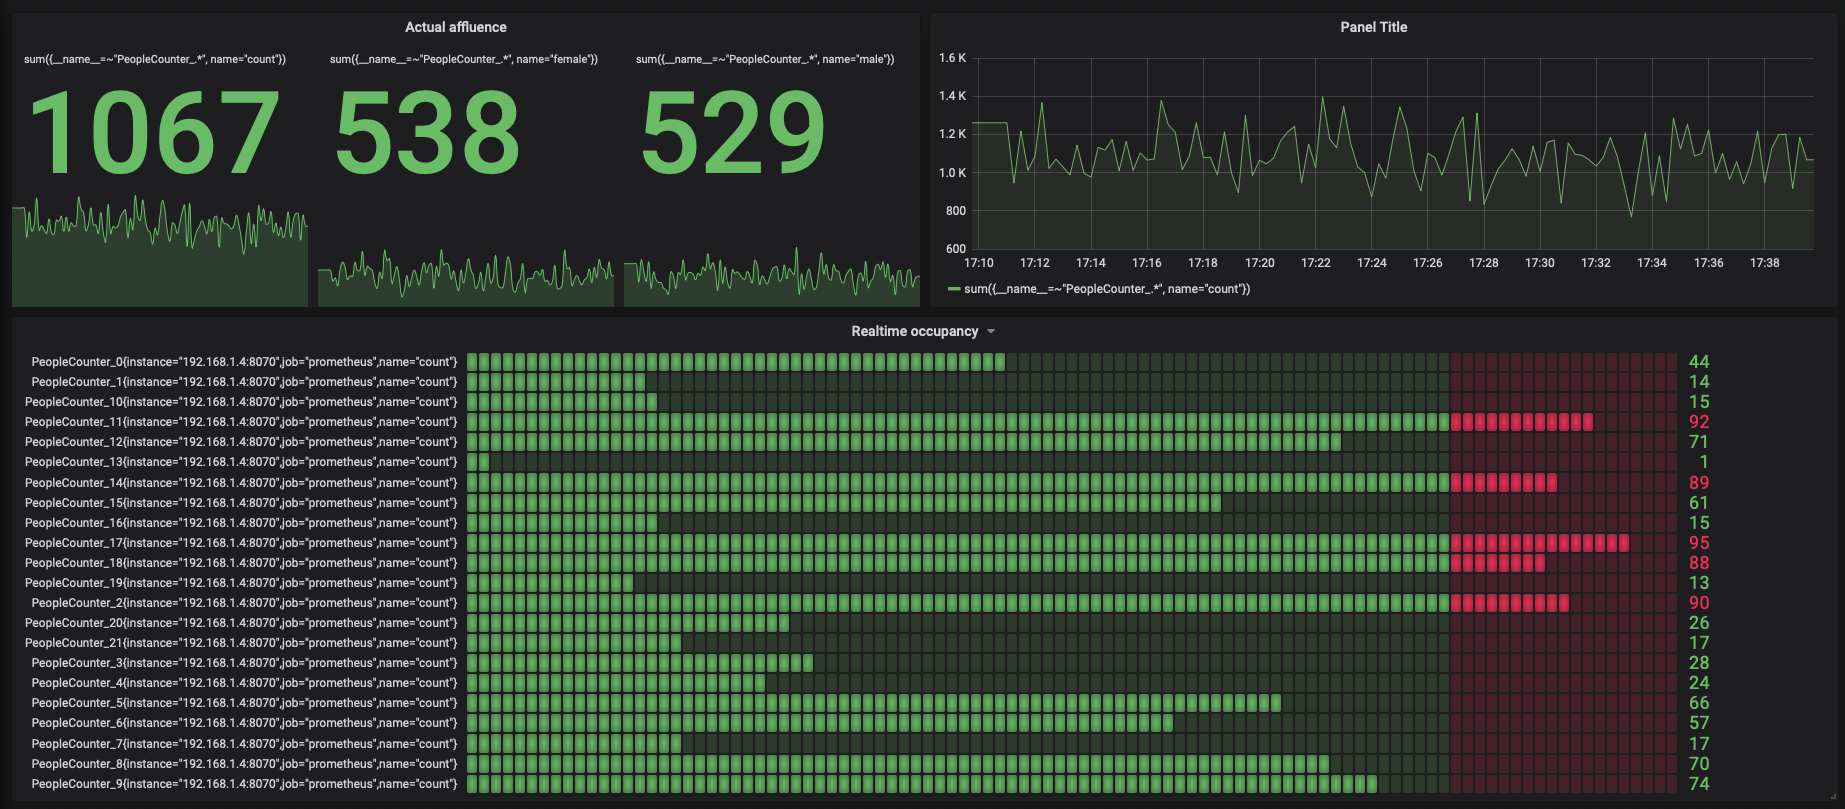
\includegraphics[width=0.7\textwidth]{Images/grafana.png}
    \caption{A dashboard created using the queries in the example above}
\end{figure}{}

\newpage
\section{Conclusions}
\subsection{FogFlow pros and cons}
Here are listed pros and cons of FogFlow. They are not related to this research project specifically, but more to a general context. Instead, in the next section is explained how well FogFlow addressed this research's problems. Finally, in the last section I propose a project that involves FogFlow and Polimi in which, I think, FogFlow will show all of its capabilities.

\subsubsection{Pros}
FogFlow, merging serverless and edge computing, it is doing what serverless computing has done but in the IoT world creating a new programming model to allow developers to focus more on the code and less on the infrastructure. It also allows to scale up the number of IoT devices (more than 1000) and reduce the latency (less than 10ms).\\
It also try to address the problem continuous changing of the requirements of an application, by allowing a so called operator to link various "functions" to create a new behaviour.

\subsubsection{Cons}
We can summarize all cons with a statement "too early to be evaluated".\\
FogFlow is a very promising tool but is on a very early stage of development, it has some important bugs that must be resolved before even thinking to deploy it in a development environment (for example some context related functionalities work only in some cases and the behaviour is not replicable).\\
Here a list of the main problems I have encountered during the development:
\begin{itemize}
    \item \textbf{Code debugging}: FogFlow does not provide any kind of debugging tool and you have to find some workarounds to be able to see what code is doing.
    \item \textbf{Not replicable behaviour}: Fog Functions are not triggered in a replicable behaviour, basically preventing the system to work properly each time is started. The problem is, in fact, related in how the Operator and the Fog Function are registered into the system.
    \item \textbf{No OTG image update}: Docker images, on which Operators are based, cannot be updated after the registration in the system.
    \item \textbf{No context queries in JS}: Using Javascript to write a Fog Function prevented me to query contexts. Instead I was able to do that in Java.
\end{itemize}
Also the programming model is not easy to understand, preventing FogFlow to be applied on new applications. I think that is mainly because it is developed by a single person, that also designed it without the support of other team members. This led to a very interesting tool but difficult to be understood.

\subsection{Results of this research}
Develop this project using FogFlow was a success, it fitted very well with the requirements and the results are promising also to think about a real implementation.\\
We successfully had the informations we were looking for and, with Fog Functions, we were capable of coding the behaviour we were looking for.\\
The downside is that FogFlow is capable of doing more than this. In a exposition there may be hundreds of sensors and there is not, geographically speaking, distribution between them, so using a tool like FogFlow is underrating its capabilities.

\subsection{\textbf{Project proposal}: Promoting social distancing in Polimi's libraries using FogFlow}
During the COVID-19 outbreak Polimi shifted most of its activities online, also closing its students' dedicated spaces.\\
Now the situation is under control and Polimi restarted to allow access to libraries and other common spaces, but with an online reservation system that now might works but in September, when students will come back (we hope) to attend lectures, the system will face a lot of difficulties due to, for example, "fake" reservations.
\subsubsection{Goals}
So the goals at which the system will aim are:
\begin{itemize}
    \item Allow students to know how much people they will find
    \item Know the total number of people inside and so preventing the access if the maximum capacity is reached
    \item Promote an equal distribution of time (some people leave their stuff for hours)
    \item Trace possible contacts people may have (respecting their privacy)
\end{itemize}
\subsubsection{When}
\begin{itemize}
    \item Using Leonardo campus as a test area
    \item We can analyse FogFlow performances (maybe we can start by showing on a screen free seats)
    \item And know more about its potential, maybe also developing new features
    \item Then, if it will be a success, expand it in other Polimi’s campuses and release it so others can implement a similar solution
\end{itemize}
\subsubsection{How}
Using ESP8266 plus a HC-SR04 (the sensor may change wrt the location where it is placed) we can detect the presence of a person and send the update to FogFlow direcly though Polimi's Wi-Fi network (we can use LoRa with a mesh configuration or LoRaWAN in other situations where we do not have Wi-Fi connectivity).\\
Later FogFlow can display the affluence data in a dashboard placed in various point of interest to let students know the best suitable place to go. Also this can be integrated into Polimi's app, maybe taking the opportunity to renew the whole app.

\begin{figure}[H]
    \centering
    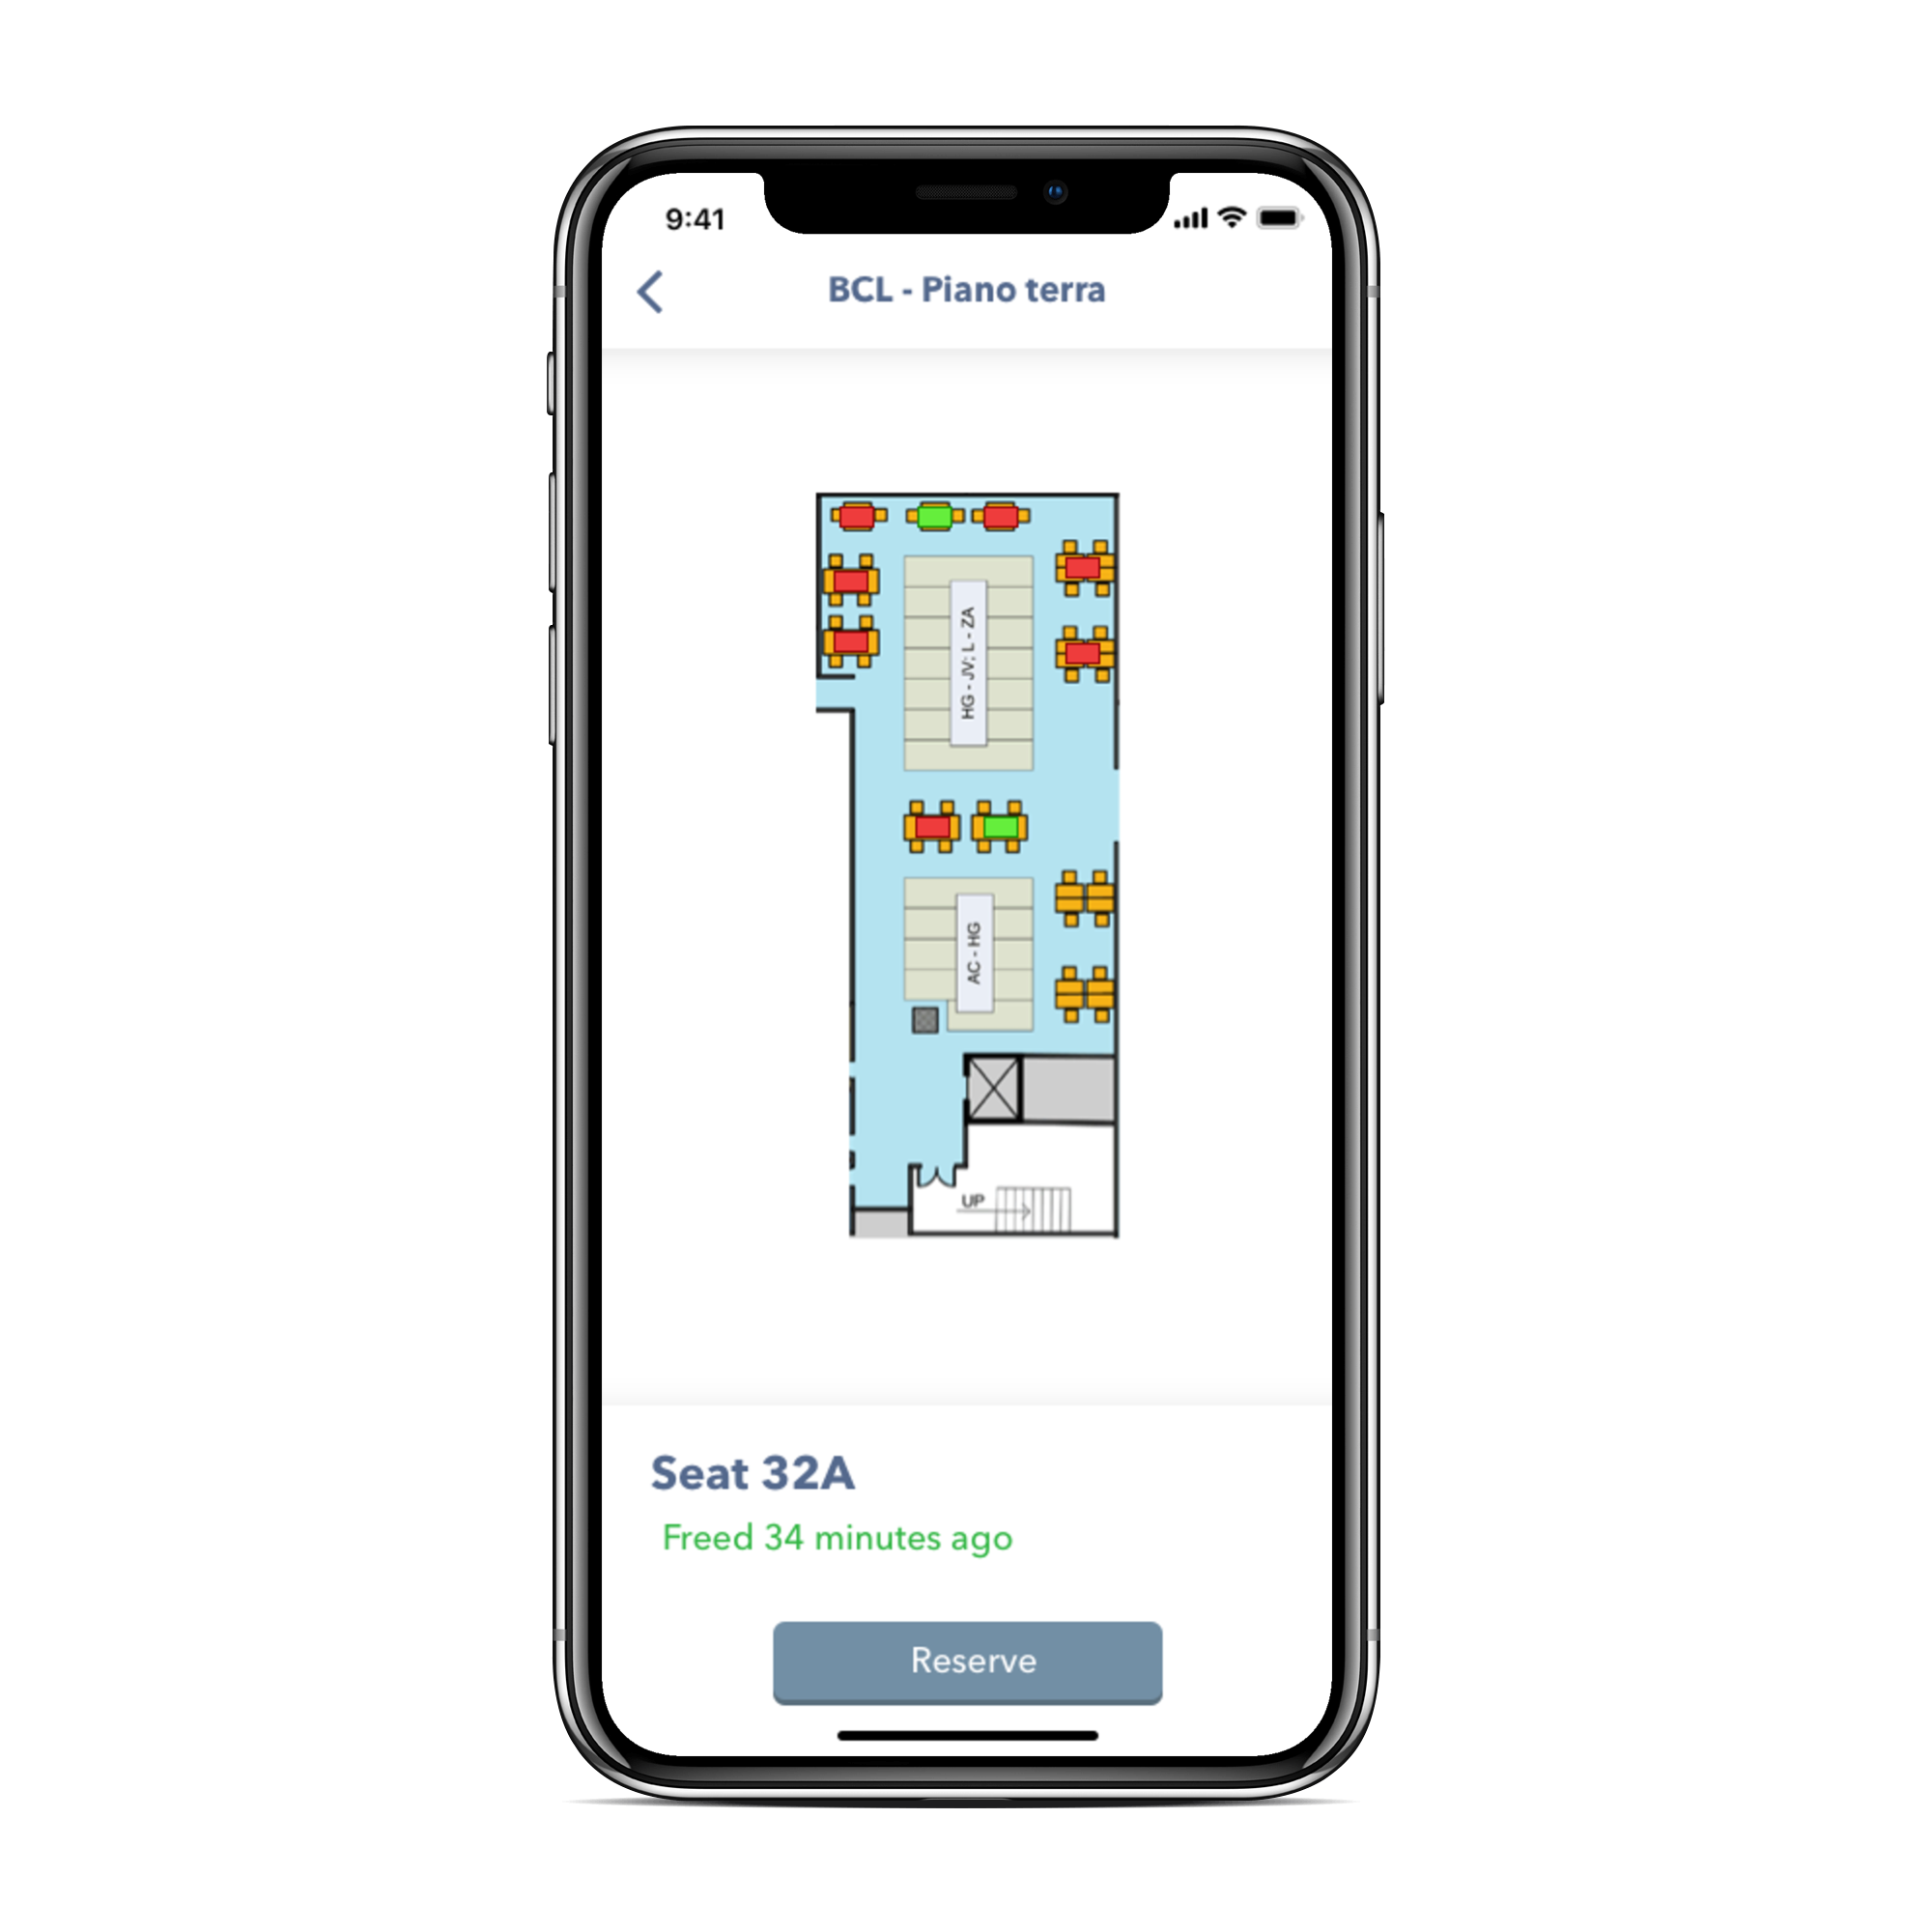
\includegraphics[width=0.7\textwidth]{Images/map.png}
    \caption{Using a map to show students the best suitable place to go}
\end{figure}{}

\bibliography{main}
\bibliographystyle{ieeetr}
\end{document}